% !TeX spellcheck = en_GB
% =================================================================
\chapter{Example Queries and Answers: A Case Study}
\label{chap:prototype_queries}
\label{chap:example_queries}

As a first step towards delineating the type of queries that should be covered by our approach,
we examine the queries used as motivating examples in Section~\ref{sec:background} more closely.
Those queries will serve as a point of reference for the analysis of the available data sources
in Chapter~\ref{chap:analysis},
and they will be generalised by the abstract framework developed in Chapter~\ref{chap:modelling}.
With that framework, we will provide a rigorous definition of the admissible queries 
that specifies their structure but does not impose any restriction on their content.

% -----------------------------------------------------------------
\section{Example Queries}
\label{sec:prototype_queries}
\label{sec:example_queries}

As already noted in Section~\ref{sec:background}, the queries introduced there
are in fact \emph{query patterns}, and we will make this distinction in the remainder
of this section. We repeat the query patterns here in order to discuss them in more depth.
%
\begin{enumerate}
  \item[\exaquery{1}]
    Who read %\todo[color=red!30]{read $\neq$ own; make clear what is meant}
    work $X$, in which manifestation and in which year?
  \item[\exaquery{2}]
    Which exemplars
%    \footnote{%
%      Conforming to the FRBR model \autocite{FRBR1998},
%      the precise wording should be \enquote{examplars of manifestations of expressions of $X$}
%      but, here and in the following,
%      we omit the intermediate entities for brevity when no misunderstanding is expected.%
%    }
    of work $X$
    were passed from one of its owners to a student?
  \item[\exaquery{3}]
    What are the relationships between the recipients of manifestation $Y$ of work $X$?
%    (or of manifestation $M$ of $W$ or of exemplar $C$ of $W$, respectively)?
  \item[\exaquery{4}]
    Which items from a collection $X$ were passed on by its owner to a family member?
  \item[\exaquery{5}]
    Which items from the holdings of library $X$ were acquired from bookseller $Y$
    between 1933 and 1945?
  \item[\exaquery{6}]
    Who participated in the sale of collection $X$?
  \item[\exaquery{7}]
    Via which paths did items from collection $X$ enter library $Y$?
  \item[\exaquery{8}]
    Which libraries own the items once owned by person $X$?
  \item[\exaquery{9}]
    Where did person $X$ acquire items and did they know the previous owners?
\end{enumerate}
%
These patterns can be turned into specific queries by instantiating each each variable with a specific object.
For example, the variable $X$
in \exaquery{2} can be instantiated with the seminal work \emph{De revolutionibus orbium coelestium}
(short: \emph{De revolutionibus}; English translation: \emph{On the Revolutions of the Heavenly Spheres}) \autocite{Kopernikus1543}
by the astronomer Nicolaus Copernicus (1473–1543).
Together with the additional specification that the owner of the book is a scientist,
we thus obtain the following query.
%
\newcommand{\Qtwoprime}{%
  \begin{enumerate}
    \item[\exaquery{2$'$}]
  %    Which exemplars of \emph{De revolutionibus} were owned by scientists who passed them on to a student?
      Which exemplars of \emph{De revolutionibus} were owned by some scientist who passed them on to a student?
  \end{enumerate}
}%
\Qtwoprime
%
It is important to note that these exemplary query patterns are not meant to be representative
for the range of queries that provenance researchers are interested in asking.
Finding a representative choice would require a systematic analysis
of queries relevant to or useful for researchers.
Such an analysis would need to comprise an extensive interview study
based on very generic questions of a predominantly open-ended nature,
requiring a labour-intensive evaluation which could easily fill a separate thesis.
As indicated above, the general framework that we will develop
is informed by the available data sources
and designed to cover a wide range of possible queries.
Hence,
it is reasonable to assume that tools developed on its basis will be helpful for provenance researchers.
In subsequent work, when our method will hopefully have been implemented in a prototype retrieval system,
the extent to which researchers' needs are served can be determined by means of a more focused user study
with more specific questions, which in turn can inform possible extensions of the framework.

% -----------------------------------------------------------------
\section{Manual Answer Retrieval}
\label{sec:manual_answering}

In order to demonstrate how a researcher could proceed (manually) when answering a query,
we consider the query~\exaquery{2$'$} from above.
An obvious way to proceed is the following.
First, our researcher finds exemplars of \emph{De revolutionibus} 
in online catalogues of libraries and library networks. For each such exemplar, they then inspect the provenance entries
that name owners who were people (not corporate bodies). Finally, our researcher will have to find those names in databases such as
authority files or Wikidata and, for each entry, search the listed professions 
and relationships to other people for the specified concept \term{Scientist} and relation \term{student}.

For example, the online catalogue (OPAC) of the Gotha Research Library of the University of Erfurt (Forschungsbibliothek Gotha) lists two printed exemplars
of \emph{De revolutionibus} \autocite{OPACDeRev}.
%\footnote{%
%  \url{https://opac.uni-erfurt.de/DB=1/CMD?ACT=SRCHA&IKT=1016&SRT=YOP&TRM=tit+de+revolutionibus+and+per+kopernikus+and+jah+15**+and+bbg+a*}%
%}
One of those bears the signature \sig{Druck~4°~00466}, and its provenance entries name the following previous owners \autocite{OPACDeRevPPN}; see also Figure~\ref{fig:OPAC_derev_provenance}:
%\footnote{%
%  \url{https://opac.uni-erfurt.de/LNG=EN/DB=1/XMLPRS=N/PPN?PPN=567506266}%
%}
%
\begin{itemize}
  \item
    Hieronymus Tilesius (1529–1566): autograph and date 1551
  \item
    NN: note, date 1553, name scraped out
  \item
    Johann Hommel (1518–1562), autograph
  \item
    Valentin Thau (1531–1575), note (greek proverb, possibly not denoting ownership)
  \item
    Ernest II, Duke of Saxe-Gotha-Altenburg (1745–1804): stamp/seal, initial
  \item
    Ducal Library, Gotha (a predecessor organisation of Gotha Research Library): stamp marking a duplicate
  \item
    Ernestine Gymnasium, Gotha: stamp
  \item
    Landesbibliothek Gotha: stamp
\end{itemize}

\begin{figure}[ht]
  \centering
  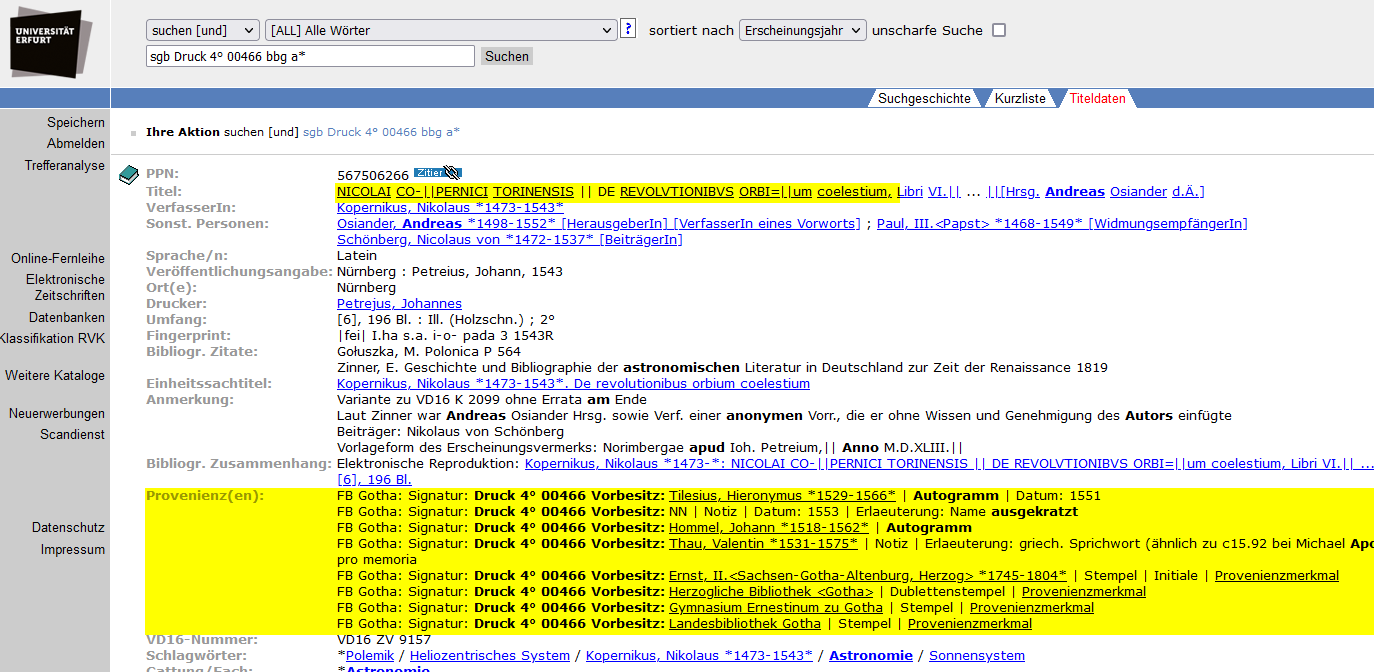
\includegraphics[width=\linewidth]{img/opac_derev_prov.png}
  \caption{University of Erfurt OPAC search result for exemplar \sig{Druck~4°~00466} of \enquote{De Revolutionibus} with provenance entries, screenshot of 2023-06-05}
  \label{fig:OPAC_derev_provenance}
\end{figure}

Our researcher can immediately decide that they can ignore the second entry (no name given) and the last three entries (corporate bodies).
For the persons named in the remaining four entries, our researcher finds the corresponding \gls{GND} records, which involves manual disambiguation in the case of Tilesius
\autocite{GNDTilesius,GNDHommel,GNDThau,GNDErnstII}.
%\footnote{%
%  \url{https://katalog.dnb.de/EN/home.html?v=plist}%
%}
On inspection of these \gls{GND} entries, it turns out that Ernest II was a regent and very probably not a scientist,
and that the other three people---Tilesius, Hommel, and Thau---had professions such as theologian,
mathematician, and astronomer, which qualifies them as scientists. Furthermore, Hommel's entry \todo{include screenshot}
contains a reference to Thau via the relation \term{student}, see Figure~\ref{fig:GND_Hommel}
(and Thau's entry contains the inverse reference to Hommel).
From this reference, our researcher can conclude that two scientists in the teacher-student relation
have both possessed the exemplar. 

\begin{figure}[ht]
  \centering
  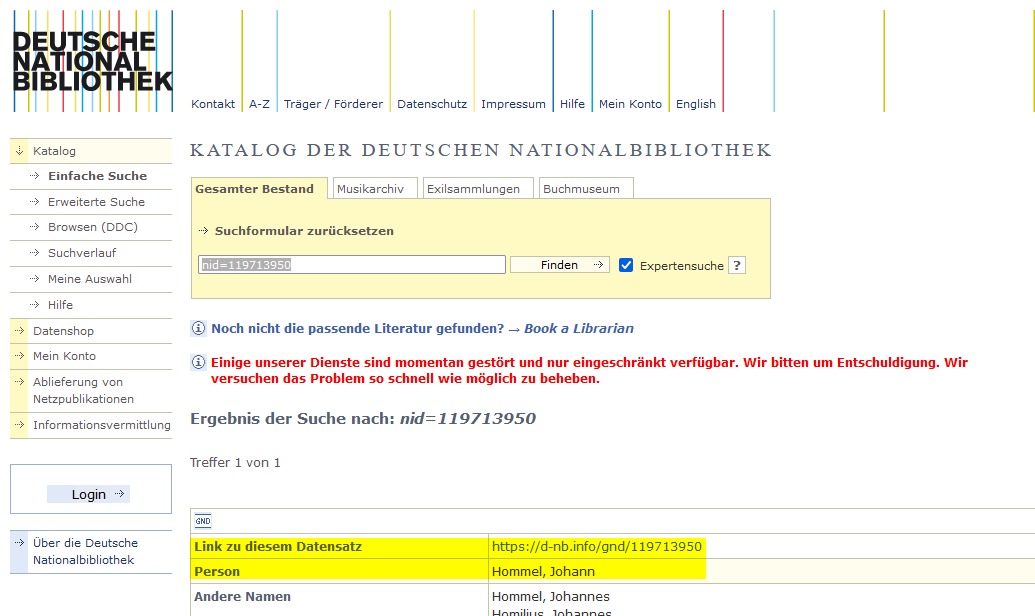
\includegraphics[width=\linewidth]{img/gnd_hommel_1.png}
  $\big[\raisebox{-1.8pt}{\rvdots}\big]$
  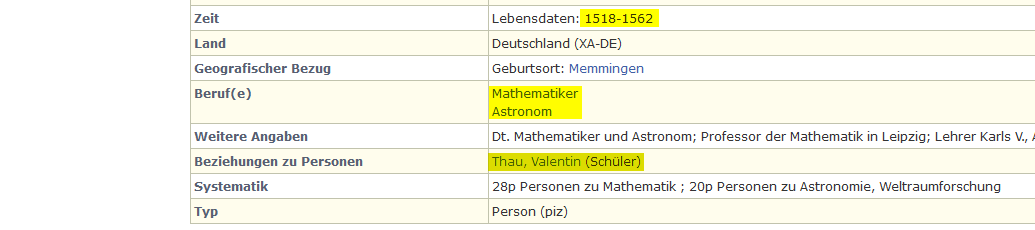
\includegraphics[width=\linewidth]{img/gnd_hommel_2.png}
  \caption{GND entry for Johann Hommel, screenshot of 2023-06-05}
  \label{fig:GND_Hommel}
\end{figure}

Unfortunately, the data available does not imply that Hommel passed the exemplar (directly) to Thau;
furthermore, the provenance entry for Thau raises doubts as to whether Thau was really an owner of the exemplar.
Therefore, the retrieved data can only be regarded as a \emph{candidate answer}
which entails the hypothesis that the found exemplar was passed from Hommel to Thau.
Our researcher can now engage in further research in order to verify that hypothesis.

\todo[think,inline]{Discuss specifics of \exaquery{1}, \exaquery{3}--\exaquery{9} (extend remarks from Section~\ref{sec:background})?}

% -----------------------------------------------------------------
\section{The Quality of Query Answers}
\label{sec:quality_of_answers}

Our simple example already illustrates that the quality of query answers
strongly depends on the quality of the underlying data,
regardless of whether answers are obtained manually or automatically. 
In particular, missing or spurious data will lead to missing or spurious answers.
Before we begin to deal with automated query answering,
we need to analyse the sources of missing or spurious data and their effects on the answers obtained.

For the sake of a principled discussion, we call the set of answers to a query obtained by some manual or automatic procedure
an \emph{answer set}, and we call the (set of) answers that the query has in reality the \emph{true answers} and the \emph{true answer set}.
In the above example, the answer set obtained by the described manual process consists of the single answer
\enquote{\sig{Druck~4°~00466}}, if we assume that our researcher interprets the data retrieved generously
(i.e., as an indication that Thau might have been an owner and might have received the book directly from Hommel)
and draws additional conclusions (i.e., that every mathematician or astronomer is a scientist).
The true answer set is not known and will most probably never be known; it is a term of rather philosophical nature.

Ideally, both answer sets should coincide.
Incomplete data may cause the answer set to exclude some true answers,
and spurious data may cause it to contain some answers that are not true.
We call the respective answers \emph{missing} and \emph{spurious}.
On the basis of our example, we can identify four distinct causes for data being incomplete or spurious,
as discussed in the following. We use the word \emph{term} as an umbrella term for concepts (such as \term{Scientist})
and relations (such as \term{student}).
%
\begin{enumerate}
  \item
    In the example, there is no information available in the \gls{GND} on whether any of the persons involved is indeed
    a \emph{scientist}. Instead, \gls{GND} provides information on more specific professions,
    e.g., for Thau and Hommel (theologian, mathematician, and astronomer).
    The information that they were scientists has to be \emph{derived} based on \emph{general knowledge
    of the world}.
    Indeed, a search in the \gls{GND} catalogue
    reveals that \gls{GND} does have an entry for the subject term \term{Wissenschaftler} (scientist) \autocite{GNDScientist}
    which, however, is used only sporadically: its 46 subordinate terms do not include, for example,
    \term{Mathematiker}, \term{Astronom}, or \term{Theologe} (mathematician, astronomer, theologian)  \autocite{GNDScientistSub}.
    
    The same effect can occur with relations instead of concepts:
    if \exaquery{2} were to ask for family members instead of collaborators or students
    but the data only supported more specific relations
    such as \term{sister} or \term{father}, then relationships using
    \term{familyMember} would need to be derived.
    Unfortunately, the cataloguing rules for \gls{GND} authority datasets do not require
    that relationships are recorded exhaustively nor using a normed vocabulary;
    see Section~\ref{sec:data_sources} for more details.
    
    In summary, terms can be missing in the data sources because
    they have not been recorded or because they are implicit in more specific terms.
    If the query uses such missing terms, then the answer set is always empty
    unless the person or machine determining the answers makes derivations based on their
    knowledge of the world.

%    Clearly, it would not be advisable to attempt adding all implicit knowledge to the data
%    because that would massively inflate the data,
%    as most terms have several superordinate concepts or relations and,
%    furthermore, implicit knowledge is not restricted to taxonomic knowledge.
%    \todo[think,inline]{Explain this further? A case for ontologies!}
  \item
    In the example, there is no information available on whether any of the owners of the exemplar
    \emph{passed it on} to another owner. Similarly,
    attempts to answer instances of Query Pattern~\exaquery{1} will have to deal
    with the problem that there is no information available as to who \emph{read} books.
    
    More generally speaking, terms can be missing in the data sources
    because they are not recorded at all, as a consequence of either a general lack of evidence
    or a general design decision for the data source. The underlying reasons can be manifold:
    for example, relationships such as who actually \emph{read} a book are very hard to confirm,
    or terms may not be part of the fixed vocabulary for a data field in a source.
    If the query uses such terms, then the answer set is always empty, as in Case~1.
  \item    
    In the example, it is possible that single owners of the exemplar or single relationships between owners
    have not been recorded because no evidence has been found yet.
    More generally, concept memberships or relationships can be missing sporadically,
    which may lead to missing answers.
  \item
    In the example, if Hommel is erroneously recorded as the owner, then the answer obtained on the grounds
    of that record is spurious.
    More generally, spurious concept memberships or relationships may lead to spurious answers.
\end{enumerate}
%
These cases reveal a striking qualitative difference concerning the effects of data incompleteness or spuriousness
on the answer set: Cases~3 and~4 have effects on single answers only, i.e., some answers are missing or spurious.
However, Cases~1 and~2 generally make \emph{all} answers missing unless further provisions are made.
Such \enquote{provisions} might include \emph{reasoning}
(e.g., deriving the implicit knowledge that Hommel was a scientist from the explicitly recorded fact that he was a mathematician)
and \emph{hypothesising} (e.g., assuming that Thau was an owner and received the book directly from Hommel).
Reasoning can be supported using semantic technologies such as (domain-specific or top-level) ontologies and related infrastructure.
A possible way to support hypothesising is to provide for the use of \emph{substitute information},
which has been addressed in the context of the \gls{SoNAR} project; see Section~\ref{sec:HNA+SoNAR}.
That is, users could be allowed to declare terms occurring in the data that may act as substitutes for certain terms used in their queries.

% Getting back to the general objective of this thesis, 
In the light of these observations,
it is appropriate to consider
query answers as \emph{candidates} that necessitate (and inspire) further research.
%as ....
For this purpose, spurious answers (in manageable numbers) are less harmful than missing answers.
Consequently, it is important to find ways to avoid missing answers without generating too many spurious answers.
In other words, it is desirable to obtain an answer set that is a slight \emph{overapproximation}
of the true answer set.

% -----------------------------------------------------------------
\section{From Manual to Automated Query Answering}
\label{sec:manual_vs_automated}

The manual process that we have described in Section~\ref{sec:manual_answering}
is cumbersome, laborious, and prone to errors and omissions for several reasons:
The search in library catalogues for exemplars of works and their provenances requires expert skills.
Catalogues with potential matches need to be selected manually,
and each catalogue needs to be queried individually, using its own search keys and syntax. 
%\todo[think]{give examples of commonalities (OPAC) and differences (discovery vs. OPAC)?}
For each retrieved exemplar, each potentially relevant provenance entry 
needs to be followed up in further data sources such as authority files,
multiplying the amount of manual work necessary.
Finally, it is not clear what an effective and efficient way to manually \enquote{explore}
relationships would be:
while it is easy to find direct relationships such as \term{student} in the view for a person's entry
in databases such as \gls{GND} or Wikidata, there are \emph{indirect} relationships
that are much harder to discover easily by hand,
e.g., \enquote{persons $P_1$ and $P_2$ are students of the same scholar}.

These considerations suggest that query answering will
strongly benefit from automated support,
which can help reduce the amount of manual work, integrate heterogeneous data sources,
incorporate background knowledge (e.g., every mathematician is a scientist),
and discover indirect relationships between entities or \enquote{substitute information}.
We envisage a retrieval system that enables researchers to formulate queries 
and which computes answers consulting data sources selected by the user.
The vocabulary used for formulating queries should be based on the vocabulary
present in the data sources, but it should also include concepts and relations
such as \term{scientist} or \term{read},
which are not recorded in the data, as discussed in
Section~\ref{sec:quality_of_answers}. The retrieval system thus needs to implement ways
to match those terms with the available vocabulary, as well as techniques
for integrating data from heterogeneous sources.
It is our general vision that the retrieval system will serve as an instrument for prospectively finding interesting
candidates that inspire further research.
In the remainder of this thesis, we want to lay the foundations and develop a precise method
that can serve as a basis for a future implementation of a retrieval system.

